% Options for packages loaded elsewhere
\PassOptionsToPackage{unicode}{hyperref}
\PassOptionsToPackage{hyphens}{url}
\PassOptionsToPackage{dvipsnames,svgnames,x11names}{xcolor}
%
\documentclass[
  11pt,
  dvipsnames,enabledeprecatedfontcommands]{scrartcl}
\usepackage{amsmath,amssymb}
\usepackage{lmodern}
\usepackage{iftex}
\ifPDFTeX
  \usepackage[T1]{fontenc}
  \usepackage[utf8]{inputenc}
  \usepackage{textcomp} % provide euro and other symbols
\else % if luatex or xetex
  \usepackage{unicode-math}
  \defaultfontfeatures{Scale=MatchLowercase}
  \defaultfontfeatures[\rmfamily]{Ligatures=TeX,Scale=1}
\fi
% Use upquote if available, for straight quotes in verbatim environments
\IfFileExists{upquote.sty}{\usepackage{upquote}}{}
\IfFileExists{microtype.sty}{% use microtype if available
  \usepackage[]{microtype}
  \UseMicrotypeSet[protrusion]{basicmath} % disable protrusion for tt fonts
}{}
\usepackage{xcolor}
\usepackage{graphicx}
\makeatletter
\def\maxwidth{\ifdim\Gin@nat@width>\linewidth\linewidth\else\Gin@nat@width\fi}
\def\maxheight{\ifdim\Gin@nat@height>\textheight\textheight\else\Gin@nat@height\fi}
\makeatother
% Scale images if necessary, so that they will not overflow the page
% margins by default, and it is still possible to overwrite the defaults
% using explicit options in \includegraphics[width, height, ...]{}
\setkeys{Gin}{width=\maxwidth,height=\maxheight,keepaspectratio}
% Set default figure placement to htbp
\makeatletter
\def\fps@figure{htbp}
\makeatother
\setlength{\emergencystretch}{3em} % prevent overfull lines
\providecommand{\tightlist}{%
  \setlength{\itemsep}{0pt}\setlength{\parskip}{0pt}}
\setcounter{secnumdepth}{5}
\newlength{\cslhangindent}
\setlength{\cslhangindent}{1.5em}
\newlength{\csllabelwidth}
\setlength{\csllabelwidth}{3em}
\newlength{\cslentryspacingunit} % times entry-spacing
\setlength{\cslentryspacingunit}{\parskip}
\newenvironment{CSLReferences}[2] % #1 hanging-ident, #2 entry spacing
 {% don't indent paragraphs
  \setlength{\parindent}{0pt}
  % turn on hanging indent if param 1 is 1
  \ifodd #1
  \let\oldpar\par
  \def\par{\hangindent=\cslhangindent\oldpar}
  \fi
  % set entry spacing
  \setlength{\parskip}{#2\cslentryspacingunit}
 }%
 {}
\usepackage{calc}
\newcommand{\CSLBlock}[1]{#1\hfill\break}
\newcommand{\CSLLeftMargin}[1]{\parbox[t]{\csllabelwidth}{#1}}
\newcommand{\CSLRightInline}[1]{\parbox[t]{\linewidth - \csllabelwidth}{#1}\break}
\newcommand{\CSLIndent}[1]{\hspace{\cslhangindent}#1}
%\documentclass{article}

% %packages
\usepackage{booktabs}
%\usepackage[left]{showlabels}
\usepackage{multirow}
\usepackage{subcaption}
\usepackage{wrapfig}
\usepackage{graphicx}
\usepackage{longtable}
\usepackage{ragged2e}
\usepackage{etex}
%\usepackage{yfonts}
\usepackage{marvosym}
\usepackage[notextcomp]{kpfonts}
\usepackage{nicefrac}
\newcommand*{\QED}{\hfill \footnotesize {\sc Q.e.d.}}
\usepackage{floatrow}
\usepackage{multicol}

\usepackage{setspace}
\usepackage[pagewise]{lineno}

\usepackage[textsize=footnotesize]{todonotes}
\newcommand{\ali}[1]{\todo[color=gray!40]{\textbf{Alicja:} #1}}
\newcommand{\mar}[1]{\todo[color=blue!40]{#1}}
\newcommand{\raf}[1]{\todo[color=olive!40]{#1}}

%\linespread{1.5}
\newcommand{\indep}{\!\perp \!\!\! \perp\!}


\setlength{\parindent}{10pt}
\setlength{\parskip}{1pt}


%language
%\usepackage{times}
\usepackage{mathptmx}
\usepackage[scaled=0.86]{helvet}
\usepackage{t1enc}
%\usepackage[utf8x]{inputenc}
%\usepackage[polish]{babel}
%\usepackage{polski}




%AMS
\usepackage{amsfonts}
\usepackage{amssymb}
\usepackage{amsthm}
\usepackage{amsmath}
\usepackage{mathtools}

\usepackage{geometry}
 \geometry{a4paper,left=35mm,top=20mm,}


%environments
\newtheorem{fact}{Fact}


% allow page breaks in equations
\allowdisplaybreaks


%abbreviations
\newcommand{\ra}{\rangle}
\newcommand{\la}{\langle}
\newcommand{\n}{\neg}
\newcommand{\et}{\wedge}
\newcommand{\jt}{\rightarrow}
\newcommand{\ko}[1]{\forall  #1\,}
\newcommand{\ro}{\leftrightarrow}
\newcommand{\exi}[1]{\exists\, {_{#1}}}
\newcommand{\pr}[1]{\ensuremath{\mathsf{P}(#1)}}
\newcommand{\ppr}[2]{\ensuremath{\mathsf{P}^{#1}(#2)}}
\newcommand{\cost}{\mathsf{cost}}
\newcommand{\benefit}{\mathsf{benefit}}
\newcommand{\ut}{\mathsf{ut}}

\newcommand{\odds}{\mathsf{Odds}}
\newcommand{\ind}{\mathsf{Ind}}
\newcommand{\nf}[2]{\nicefrac{#1\,}{#2}}
\newcommand{\R}[1]{\texttt{#1}}
\newcommand{\prr}[1]{\mbox{$\mathtt{P}_{prior}(#1)$}}
\newcommand{\prp}[1]{\mbox{$\mathtt{P}_{posterior}(#1)$}}



\newtheorem{q}{\color{blue}Question}
\newtheorem{lemma}{Lemma}
\newtheorem{theorem}{Theorem}
\newtheorem{corollary}{Corollary}[fact]


%technical intermezzo
%---------------------

\newcommand{\intermezzoa}{
	\begin{minipage}[c]{13cm}
	\begin{center}\rule{10cm}{0.4pt}



	\tiny{\sc Optional Content Starts}
	
	\vspace{-1mm}
	
	\rule{10cm}{0.4pt}\end{center}
	\end{minipage}\nopagebreak 
	}


\newcommand{\intermezzob}{\nopagebreak 
	\begin{minipage}[c]{13cm}
	\begin{center}\rule{10cm}{0.4pt}

	\tiny{\sc Optional Content Ends}
	
	\vspace{-1mm}
	
	\rule{10cm}{0.4pt}\end{center}
	\end{minipage}
	}
	
	
%--------------------






















\newtheorem*{reply*}{Reply}
\usepackage{enumitem}
\newcommand{\question}[1]{\begin{enumerate}[resume,leftmargin=0cm,labelsep=0cm,align=left]
\item #1
\end{enumerate}}

\usepackage{float}

% \setbeamertemplate{blocks}[rounded][shadow=true]
% \setbeamertemplate{itemize items}[ball]
% \AtBeginPart{}
% \AtBeginSection{}
% \AtBeginSubsection{}
% \AtBeginSubsubsection{}
% \setlength{\emergencystretch}{0em}
% \setlength{\parskip}{0pt}






\usepackage[authoryear]{natbib}

%\bibliographystyle{apalike}



\usepackage{tikz}
\usetikzlibrary{positioning,shapes,arrows}

\ifLuaTeX
  \usepackage{selnolig}  % disable illegal ligatures
\fi
\IfFileExists{bookmark.sty}{\usepackage{bookmark}}{\usepackage{hyperref}}
\IfFileExists{xurl.sty}{\usepackage{xurl}}{} % add URL line breaks if available
\urlstyle{same} % disable monospaced font for URLs
\hypersetup{
  pdftitle={Awareness Growth in Bayesian Networks:},
  colorlinks=true,
  linkcolor={Maroon},
  filecolor={Maroon},
  citecolor={Blue},
  urlcolor={blue},
  pdfcreator={LaTeX via pandoc}}

\title{Awareness Growth in Bayesian Networks:}
\usepackage{etoolbox}
\makeatletter
\providecommand{\subtitle}[1]{% add subtitle to \maketitle
  \apptocmd{\@title}{\par {\large #1 \par}}{}{}
}
\makeatother
\subtitle{The Role of Structural Assumptions}
\author{}
\date{\vspace{-2.5em}July 28, 2022}

\begin{document}
\maketitle

\doublespace

\emph{Wordcount (including footnotes)}: 5,392

\begin{abstract}
We examine different counterexamples to Reverse Bayesianism, a popular theory 
that addresses the problem of awareness growth. We agree with the general skepticism toward Reverse Bayesianism, but submit that the problem of awareness growth cannot be tackled in an algorithmic manner, because subject-matter, structural assumptions need to be made explicit. Thanks to their ability to express probabilistic dependencies, we illustrate how Bayesian networks can help to model awareness growth in the Bayesian framework. 
\end{abstract}

\doublespace
\linenumbers

\hypertarget{introduction}{%
\section{Introduction}\label{introduction}}

Learning is modeled in the Bayesian framework by the rule of
conditionalization. This rule posits that the agent's new degree of
belief in a proposition \(H\) after a learning experience \(E\) should
be the same as the agent's old degree of belief in \(H\) conditional on
\(E\). That is, \[\ppr{E}{H}=\pr{H \vert E},\] where \(\pr{}\)
represents the agent's old degree of belief (before the learning
experience \(E\)) and \(\ppr{E}{}\) represents the agent's new degree of
belief (after the learning experience \(E\)).

Both \(E\) and \(H\) belong to the agent's algebra of propositions. This
algebra models the agent's awareness state, the propositions taken to be
live possibilities. Conditionalization never modifies the algebra and
thus makes it impossible for an agent to learn something they have never
thought about. Even before learning about \(E\), the agent must already
have assigned a degree of belief to any proposition conditional on
\(E\). This picture commits the agent to the specification of their
`total possible future experience' (Howson, 1976), as though learning
was confined to an `initial prison' (Lakatos, 1968).

But, arguably, the learning process is more complex than what
conditionalization allows. Not only do we learn that some propositions
that we were entertaining are true or false, but we may also learn new
propositions that we did not entertain before. Or we may entertain new
propositions---without necessarily learning that they are true or
false---and this change in awareness may in turn change what we already
believe. How should this more complex learning process be modeled by
Bayesianism? Call this the problem of awareness growth.

The algebra of propositions need not be so narrowly construed that it
only contains propositions that are presently under consideration. The
algebra may also contain propositions which, though outside the agent's
present consideration, are still the object, perhaps implicitly, of
certain dispositions to believe.\footnote{Roussos (2021) notes that, for
  the sake of clarity, the problem of awareness growth should only
  address propositions which agents are \emph{truly} unaware of (say new
  scientific theories), not propositions that were temporarily forgotten
  or set aside. This is a helpful clarification to keep in mind,
  although the recent literature on the topic does not make a sharp a
  distinction between true unawareness and temporary unawareness.} But
even this expanded algebra will have to be revised sooner or later. The
algebra of propositions could in principle contain anything that could
possibly be conceived, expressed, thought of. Such a rich algebra would
not need to change at any point, but this is an implausible model of
ordinary agents with bounded resources such as ourselves.

Critics of Bayesianism and sympathizers alike have been discussing the
problem of awareness growth under different names for quite some time,
at least since the eighties. This problem arises in a number of
different contexts, for example, new scientific theories (Chihara, 1987;
Earman, 1992; Glymour, 1980), language changes and paradigm shifts
(Williamson, 2003), and theories of induction (Zabell, 1992). A proposal
that has attracted considerable scholarly attention in recent years is
Reverse Bayesianism (Bradley, 2017; Karni \& Vierø, 2015; Wenmackers \&
Romeijn, 2016). The idea is to model awareness growth as a change in the
algebra while ensuring that the proportions of probabilities of the
propositions shared between the old and new algebra remain the same in a
sense to be specified.

Let \(\mathcal{F}\) be the initial algebra of propositions and let
\(\mathcal{F}^+\) the algebra after the agent's awareness state has
grown. Both algebras contain the contradictory and tautologous
propositions \(\perp\) and \(\top\), and they are closed under
connectives such as disjunction \(\vee\), conjunction \(\wedge\) and
negation \(\neg\). Denote by \(X\) and \(X^+\) the subsets of these
algebras that contain only basic propositions, namely those without
connectives. \textbf{Reverse Bayesianism} posits that the ratio of
probabilities for any basic propositions \(A\) and \(B\) in both \(X\)
and \(X^+\)---the basic propositions shared by the old and new
algebra---remain constant through the process of awareness growth:
\[\frac{\pr{A}}{\pr{B}} = \frac{\ppr{+}{A}}{\ppr{+}{B}},\] where
\(\pr{}\) represents the agent's degree of belief before awareness
growth and \(\ppr{+}{}\) represents the agent's degree of belief after
awareness growth.

Reverse Bayesianism is an elegant theory that manages to cope with a
seemingly intractable problem. As the awareness state of an an agent
grows, the agent would prefer not to throw away completely the epistemic
work they have done previously. The agent may desire to retain as much
of their old degrees of beliefs as possible. Reverse Bayesianism
provides a simple recipe to do that. It also coheres with the
conservative spirit of Bayesian conditionalization which preserves the
old probability distribution conditional on what is learned.

Unfortunately, Reverse Bayesianism does not deliver the intuitive
results in all cases. There is no shortage of counterexamples against it
in the recent philosophical literature (Mathani, 2020; Steele \&
Stefánsson, 2021). In addition, attempts to extent traditional arguments
in defense of Bayesian conditionalization to the case of awareness
growth seem to hold little promise (Pettigrew, forthcoming). If the
consensus in the literature is that Reverse Bayesianism is not the right
theory of awareness growth, what theory (if any) should replace it?

Here we offer a diagnosis of what is wrong with Reverse Bayesianism and
outline an alternative proposal. The problem of awareness growth---we
hold---cannot be tackled in an algorithmic manner because subject-matter
assumptions, both probabilistic and structural, need to be made
explicit. So any theory of awareness growth cannot be a purely formal
theory. This does not mean, however, we should give up on probability
theory altogether in this context. Thanks to its ability to express
probabilistic dependencies, we think that the theory of Bayesian
networks can help to model awareness growth in the Bayesian framework.
We illustrate this claim as we examine different counterexamples to
Reverse Bayesianism.

\hypertarget{expansion}{%
\section{Expansion}\label{expansion}}

A common set of cases of awareness growth are usually referred in the
literature with the label \emph{awareness expansion}. A precise
definition of expansion can be tricky to provide, but a rough
characterization will suffice here. Suppose, as is customary,
propositions are interpreted as sets of possible worlds, where the set
of all possible worlds is the possibility space. Awareness expansion
occurs when a new proposition is added to the algebra and its
interpretation includes possible worlds not in the original possibility
space. So the addition of the new proposition causes the original space
of possibilities to expand.

Perhaps the most straightforward example of awareness expansion occurs
when you become aware of a new explanation for the evidence at your
disposal which you had not considered before. This can happen in many
fields of inquiry: medicine, law, science, everyday affairs. Here is a
scenario by Steele \& Stefánsson (2021):

\begin{quote}
\textsc{Friends}: Suppose you happen to see your partner enter your best
friend's house on an evening when your partner had told you she would
have to work late. At that point, you become convinced that your partner
and best friend are having an affair, as opposed to their being warm
friends or mere acquaintances. You discuss your suspicion with another
friend of yours, who points out that perhaps they were meeting to plan a
surprise party to celebrate your upcoming birthday---a possibility that
you had not even entertained. Becoming aware of this possible
explanation for your partner's behaviour makes you doubt that she is
having an affair with your friend, relative, for instance, to their
being warm friends. (Steele \& Stefánsson, 2021, sec. 5, Example 2)
\end{quote}

\doublespace

\noindent Initially, the algebra only contained the hypotheses `my
partner and my best friend met to have an affair' (\textit{Affair}) and
`my partner and my best friend met as friends or acquaintances'
(\textit{Friends/acquaintances}). These were the only explanations you
considered for your evidence, namely that your partner and your best
friend met one night without telling you (\textit{Secretive}). Given
this evidence, \textit{Affair} is more probable than
\textit{Friends/acquaintances}:\footnote{This assumes that the prior
  probabilities of the two hypotheses were not strongly skewed in one
  direction. If you were initially nearly certain your partner could not
  possibly have an affair, even the fact they behaved very secretively
  or lied to you might not affect the probability of the two hypotheses.}
\[\pr{\textit{Affair} \vert  \textit{Secretive} }> \pr{\textit{Friends/acquaintances} \vert \textit{Secretive}} \tag{>}.\]
When the algebra changes, a new hypothesis is added which you had not
considered before: your partner and your best friends met to plan a
surprise party for your upcoming birthday (\textit{Surprise}). This
hypothesis seems to be a much better explanation. So, given the same
evidence, the hypothesis \textit{Surprise} is more likely than the
hypothesis \textit{Affair}:
\[\ppr{+}{ \textit{Surprise} \vert \textit{Secretive}}> \ppr{+}{ \textit{Affair} \vert \textit{Secretive}}.\]
And since \textit{Surprise} implies
\textit{Friends/acquaintances}---after all, in order to prepare a
surprise party, your partner and best friend have to be at least
acquaintances--- \textit{Friends/acquaintances} is now more likely than
\textit{Affair}:
\[\ppr{+}{\textit{Affair} \vert  \textit{Secretive} } < \ppr{+}{\textit{Friends/acquaintances} \vert \textit{Secretive}}. \tag{<}\]

As Steele \& Stefánsson note, the conjunction of (\(>\)) and (\(<\))
violates Reverse Bayesianism. But, they also note, a quick fix is
available. For consider the following condition, called
\textbf{Awareness Rigidity}: \[\ppr{+}{A \vert T^*}=\pr{A},\] where
\(T^*\) corresponds to a proposition that picks out, from the vantage
point of the new awareness state, the entire possibility space before
the episode of awareness growth. Awareness rigidity establishes that,
once a suitable proposition \(T^*\) is identified, the old probability
assignments can be kept conditional on \(T^*\). In our running example,
\(\neg\textit{Surprise}\) is the suitable proposition \(T^*\):
\emph{that} there were was no surprise party in the making picks out the
original possibility space in its entirety. After all, before awareness
growth, the eventuality that your partner and best friend could be
organizing a surprise for you had been tacitly ruled out. So,
conditional on \(\neg\textit{Surprise}\), no probability assignment
should change, including the probability of \textit{Affair}. Thus,
\[\ppr{+}{\textit{Affair} \vert  \textit{Secretive} \& \neg\textit{Surprise} } > \ppr{+}{\textit{Friends/acquaintances} \vert \textit{Secretive} \& \neg\textit{Surprise}}. \]

Steele and Stefansson, however, go on to show that Awareness Rigidity
does not hold in other cases, what they call awareness refinement. But
before considering them, it is important to understand why Awareness
Rigidity is an adequate principle to govern awareness growth in
expansion cases. As we shall soon see, Bayesian networks helps to model
these cases more precisely. A Bayesian network is a compact formalism to
represent probabilistic dependencies. A Bayesian network consists of a
direct acyclic graph (DAG) accompanied by a probability distribution.
The nodes in the graph represent random variables that can take
different values. We will use `nodes' and `variables' interchangeably.
The nodes are connected by arrows, but no loops are allowed, hence the
name direct acyclic graph. Bayesian networks are relied upon in many
fields, but have been rarely deployed to model awareness growth (the
exception is Williamson (2003)). We think instead they are a good
framework for this purpose. Awareness growth can be modeled as a change
in the graphical network---nodes and arrows are changed, added or
erased---as well as a change in the probability distribution from the
old to the new network.

To model \textsc{Friends} with Bayesian networks, we start with this
graph, which is the usual hypothesis-evidence idiom (Fenton, Neil, \&
Lagnado, 2013):

\begin{center}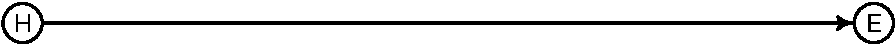
\includegraphics[width=0.5\linewidth,height=0.5\textheight]{ReplyToSteeleStefansson5_files/figure-latex/heDAG-prel-1} \end{center}

\noindent where \(H\) is the hypothesis node and \(E\) the evidence
node. If an arrow goes from \(H\) to \(E\), the full probability
distribution associated with the Bayesian network is defined by two
probability tables.\footnote{A major point of contention in the
  interpretation of Bayesian networks is is the meaning of the directed
  arrows. They could be interpreted causally---as though the direction
  of causality proceeds from the events described by the hypothesis to
  event described by the evidence---but they need not be; see footnote
  \ref{footnote:causation}.} One table defines the prior probabilities
for all the states of \(H\), and another table defines the conditional
probabilities of the form \(\pr{E=e \vert H=h}\), where uppercase
letters represent the variables (nodes) and lower case letters represent
the values of these variables. These two probability tables are
sufficient to specify the full probability distribution.

Initially, before awareness growth, the hypothesis \(H\) takes only two
values, \textit{Friends/acquaintances} and \textit{Affair}. These two
values are meant to be exhaustive. So, initially, \textit{Affair}
functions as the negation of \textit{Friends/acquaintances}, or vice
versa. After awareness growth---specifically, awareness expansion---the
two values of te node \(H\) are no longer considered exhaustive. The
node now has a third value: \textit{Surprise}. The rest of the structure
of the network remains intact.

So, expansion simply consists in the addition of an extra value in one
of the nodes of the network. Specifically, in \textsc{Friends}, the
extra value was added to the upstream node \(H\). This addition may
require a change in the probability table for the conditional
probabilities \(\pr{E=e \vert H=h}\). However, for all values \(e\) and
\(h\) of upstream node \(H\) and downstream node \(E\) in the old
network, the following constraint holds:
\[\frac{\pr{E=e \vert H=h}}{\pr{E=e \vert H=h}} = \frac{\ppr{+}{E=e \vert H=h}}{\ppr{+}{E=e \vert H=h}}. \tag{C}\]
Constraint (C) is a restricted variant of Reverse Bayesianism that only
applies to the conditional probabilities in the probability table for
the evidence-hypothesis Bayesian network.

The same approach can be adopted to handle a counterexample to Reverse
Bayesianism by Mathani (2020). It goes like this:

\begin{quote}
\textsc{Tenant}: Suppose that you are staying at Bob's flat which he shares with his landlord. You know
that Bob is a tenant, and that there is only one landlord, and that this landlord also
lives in the flat. In the morning you hear singing coming from the shower room, and
you try to work out from the sounds who the singer could be. At this point you have
two relevant propositions that you consider possible ... $Landlord$ standing for the possibility that the landlord is the singer, and $Bob$ standing for the possibility that Bob is the singer  \dots  Because you know that Bob is a tenant in the flat, you also have a credence in the proposition $Tenant$ that the singer is a tenant. Your credence in $Tenant$ is the same as your credence in $Bob$, for given your state of awareness these two propositions are equivalent ... Now let's suppose the possibility suddenly occurs to you that there might be another tenant living in the same flat  ($Other$).
\end{quote}

\doublespace

\noindent Initially, you thought the singer could either be the landlord
or Bob, the tenant. Then you come to the realization that a third person
could be the singer, another tenant. Before awareness growth, that Bob
is in the shower and that a tenant is in the shower are equivalent
descriptions. After awareness growth, this equivalence breaks down.

Why is this scenario problematic for Reverse Bayesianism? Suppose, after
you hear singing in the shower, you become sure someone is in there, but
you cannot tell who. So \(\pr{Landlord} = \pr{Bob} = 1/2\), and since
\(Bob\) and \(Tenant\) are equivalent, also \(\pr{Tenant}\) = 1/2. Now,
\(Landlord\), \(Bob\) and \(Tenant\) are all propositions that you were
originally aware of, and thus Reverse Bayesianisn requires that their
assigned probabilities should remain in the same proportion after your
awareness grows. But note that \(Other\) entails \(Tenant\) and \(Bob\)
and \(Other\) are disjoint, so it follows that \(\ppr{+}{Other}\) must
have zero probability.\footnote{If \(\ppr{+}{Other}>0\), the proportion
  of \(Tenant\) to \(Landlord\) or the proportion of \(Bob\) to
  \(Landlord\) should change.} This is an undesired outcome that rules
out the possibility that there could be a third person in the
shower.\footnote{Awareness Rigidity is no of help either because it
  would require that
  \(\ppr{+}{Landlord \vert Landlord \vee Tenant}=\ppr{+}{Bob \vert Landlord \vee Tenant}\)
  both equal \(1/2\), thus forcing
  \(\ppr{+}{Other \vert Landlord \vee Tenant}\) to zero.}

In \textsc{Tenant}, it is natural to assign \(1/3\) to \(Landlord\),
\(Bob\) and \(Other\) after awareness growth. That someone is singing in
the shower is evidence that someone must be in there, but without any
more discriminating evidence, each person should be assigned the same
probability. Consequently, a probability of 2/3 should be assigned to
\(Tenant\). On this picture, the proportion of \(Landlord\) to
\(Tenant\) changes from 1:1 (before awareness growth) to 1:2 (after
awareness growth).

Bayesian networks can help to model this scenario. We start with the
following graph:

\begin{center}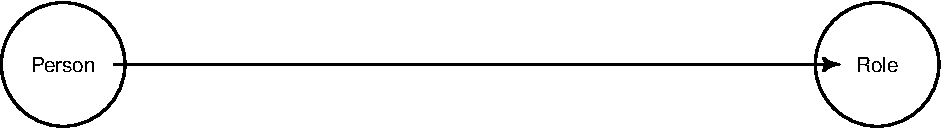
\includegraphics[width=0.5\linewidth,height=0.3\textheight]{ReplyToSteeleStefansson5_files/figure-latex/tenantsDAG-new-1} \end{center}

\noindent Initially, the upstream node \(Person\) has two possible
states, representing who is in the bathroom singing:
\textit{landlord-person} and \(bob\). To simplify things, the assumption
here is that the evidence of singing has already ruled out the
possibility that no one would be in the shower. The downstream node
\(Role\) has also two values, \(landlord\) and \(tenant\). After your
awareness grows, the upstream node \(Person\) should now have one more
possible state, \(other\).

The scenarios \textsc{Friends} and \textsc{Tenant} are structurally
identical as far as their modeling using Bayesian networks. So, if
constraint (C) holds in \textsc{Friends}, as seen earlier, it must also
hold in \textsc{Tenant}. This is precisely what happens. For these
ratios remain fixed:

\[\frac{\pr{\textit{Role}=\textit{landlord} \vert \textit{Person}=\textit{landlord}}}{\pr{\textit{Role}=\textit{landlord} \vert \textit{Person}=\textit{bob}}} = \frac{\ppr{+}{\textit{Role}=\textit{landlord} \vert \textit{Person}=\textit{landlord}}}{\ppr{+}{\textit{Role}=\textit{landlord} \vert \textit{Person}=\textit{bob}}} = 1/0\]

\[\frac{\pr{\textit{Role}=\textit{tenant} \vert \textit{Person}=\textit{landlord}}}{\pr{\textit{Role}=\textit{tenant} \vert \textit{Person}=\textit{bob}}} = \frac{\ppr{+}{\textit{Role}=\textit{tenant} \vert \textit{Person}=\textit{landlord}}}{\ppr{+}{\textit{Role}=\textit{tenant} \vert \textit{Person}=\textit{bob}}} = 0/1\]

The upshot of this discussion is this. Awareness expansion can be
modeled by changes in the Bayesian network used to represent the
epistemic state of the agent. The structure of the network does not
change, but values are added to the upstream nodes. (We will consider
changes to the downstream node shortly.) This addition can be carried
while satisfying a restricted version of Reverse Bayesian, what we
called constraint (C). This constraint outperforms both Reverse
Bayesianism (which fails in \textsc{Friends}) and Awareness Rigidity
(which fails in \textsc{Tenant}).

What would happen is the extra value is added to the downstream node in
the hypothesis-evidence network? Consider a variation of
\textsc{Friends}. Suppose that the evidence node \(E\) could initially
take only two values, say \textit{Secretive} and \textit{Public}. You
then realize the evidence node could also take a third value, say
\textit{Ambigous}. This realization mandate a change in the old
conditional probabilities \(\pr{E=e \vert H=h}\). Since
\textit{Secretive} and \textit{Public} were initially considered
exhaustive,

Since the change is downstream the old conditional probabilities
\(\pr{E=e \vert H=h}\) would remain the same, and thus \emph{a
fortiori}, constraint (C) would be satisfied.

outperformes the same result as Awareness Rigidity, but more easily
applies to the conditional probabilities that are needed in the
probability tables of Bayesian Networks. The challenge now is to develop
a systematic method to determine when constraint (C) is satisfied and
when it fails. The structure of the Bayesian network will be our guide.
This will afford us a firmer foundation to develop a general theory of
awareness growth.

\hypertarget{refinement}{%
\section{Refinement}\label{refinement}}

\label{sec:structural-both}

We turn now from cases of awareness expansion to cases of awareness
refinement. In the framework of Bayesian networks, expansion consisted
in added values to nodes in the network. Refinement, instead, can be
modeled by adding nodes to the network without necessarily add any new
values to the existing nodes. Intuitively, refinement takes place when
an epistemic agent acquires a more-fined grained picture of the
situation, say instead of thinking that the political spectrum is
divided into liberal and conservatives, the political spectrum can be
further divided into traditional-liberal, new-liberal,
traditional-conservative and new-conservative. The political spectrum is
still divided into liberal and conservative---not expansion
occurred---but these two categories have been further refined.

Although there is no shortage of counterexamples to Reverse Bayesianism
when it comes to awareness refinement, we begin with our own. This will
allow us to underscore the role of subject-matter assumptions in
theorizing about awareness growth. Consider the following scenario:

\begin{quote}
\textsc{Lighting:} You have evidence that favors a certain hypothesis, say a witness 
saw the defendant around the crime scene. You give some weight to this evidence. 
In your assessment, that the defendant was seen around the crime scene (your evidence) raises the probability that the defendant was actually there (your hypothesis). But now you ask, what if it was dark when the witness saw the defendant? In light of your realization that it could have been dark, you wonder whether (and if so how) you should change the probability that you assigned to the hypothesis that the defendant was around the crime scene.
\end{quote}

As your awareness grows, you do not learn anything specific about the
lighting conditions, neither that they were bad nor that they were good.
You simply wonder what they were, a variable you had previously not
considered. So no Bayesian updating takes place in the strict sense,
although broadly speaking some new information has been
introduced.\footnote{HERE EXPLAIN DIFFERENCE WITH STEELE AND STEFANSSON.
  The process of awareness growth in \textsc{Lighting} adds only one
  extra variable, lighting conditions, while \textsc{Movies} adds two
  extra variables, language difficulty and whether the owner is
  simple-minded or not. Further, \textsc{Movies} contains a clear-cut
  case of learning, that the owner \emph{is} simple-minded. This is not
  so in \textsc{Lighting}. Strictly speaking, you are learning that it
  is \emph{possible} that the lighting conditions were bad. However, you
  are not conditioning on the proposition `the lighting conditions were
  bad' or `the lighting conditions were good'. So you are not learning
  about the lighting conditions in the sense in which learning is
  understood in this paper.} Something has changed in your epistemic
state---you have a more fine-grained assessment of what could have
happened---but it is not clear what you should do in this scenario.
Since the lighting conditions could have been bad but could also have
been good, perhaps you should just stay put until you learn something
more specific.

In what follows, we illustrate how Bayesian networks helps to model what
is going on in \textsc{Lighting} and conclude that you should probably
revise downward your confidence in the hypothesis that the defendant was
around the crime scene. The starting point of our analysis is the usual
hypothesis-evidence idiom, repeated below for convenience:

\begin{center}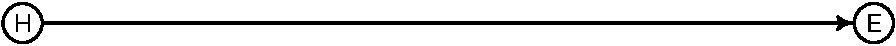
\includegraphics[width=0.5\linewidth,height=0.5\textheight]{ReplyToSteeleStefansson5_files/figure-latex/heDAG-1} \end{center}

\noindent Since you trust the evidence, you think that the evidence is
more likely under the hypothesis that the defendant was present at the
crime scene than under the alternative hypothesis:
\[\pr{\textit{E=seen} \vert \textit{H=present}} > \pr{\textit{E=seen} \vert \textit{H=absent}}\]
The inequality is a qualitative ordering of how plausible the evidence
is in light of competing hypotheses. No matter the numbers, by the
probability calculus, it follows that the evidence raises the
probability of the hypothesis \textit{H=present}.

Now, as you wonder about the lighting conditions, the graph should be
amended:

\begin{center}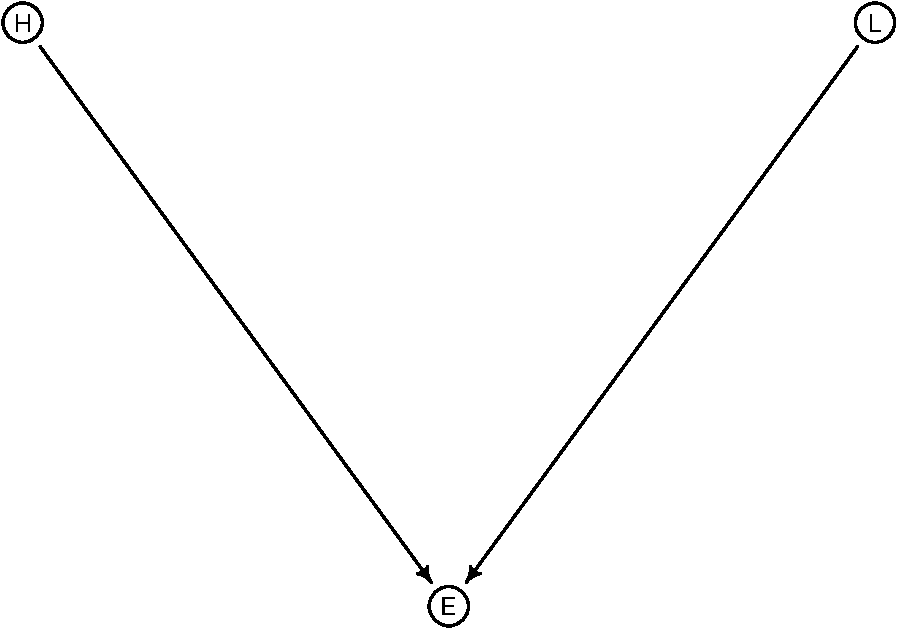
\includegraphics[width=0.5\linewidth,height=0.3\textheight]{ReplyToSteeleStefansson5_files/figure-latex/lighting2DAG-1} \end{center}

\noindent where the node \(L\) can have two values, \textit{L=good} and
\textit{L=bad}. Commonsense as well as psychological findings suggest
that when the visibility deteriorates, people's ability to identify
faces worsen. So a plausible way to modify your assessment of the
evidence is as follows:
\[\ppr{+}{\textit{E=seen} \vert \textit{H=present} \wedge \textit{L=good}} > \ppr{+}{\textit{E=seen} \vert \textit{H=absent} \wedge \textit{L=good}}\]
\[\ppr{+}{\textit{E=seen} \vert \textit{H=present} \wedge \textit{bad}} = \ppr{+}{\textit{E=seen} \vert \textit{H=absent} \wedge \textit{L=bad}}\]

\noindent In words, if the lighting conditions were good, you still
trust the evidence like you did before (first line), but if the lighting
conditions were bad, you regard the evidence as no better than chance
(second line). These probabilistic constraints are plausible, but should
ultimately be grounded on verifiable empirical regularities.

Despite the change in awareness, you have not learned anything in the
strict sense. Your new stock of evidence does not contain neither the
information that the lighting conditions were bad nor that they were
good. But the Bayesian network structure that represents your epistemic
state is now more fine-grained. The network contains the new variable
\(L\) which it did not contain prior to the episode of awareness growth.
In addition---and this is the crucial point---the new variable bears
certain \emph{structural relationships} with the variables \(H\) and
\(E\). The graphical network represents a direct probabilistic
dependency between the lighting conditions \(L\) and the witness sensory
experience \(E\), but does not allow for any direct dependency between
the lighting conditions and the fact that the defendant was (or was not)
at the crime scene. There is no direct arrow between the nodes \(L\) and
\(H\). This structure of dependencies captures our causal intuitions
about the scenario: the lighting conditions do affect what the witness
could see, but do not directly affect what the defendant might have have
done.

Without Bayesian networks, episodes of awareness growth could only be
modeled by the addition of new propositions that were not previously in
the algebra. But this approach would fail to capture crucial
information. When awareness growth takes place against the background of
an intuitive causal structure of the world---as in the case of
\textsc{Lighting}---this structure should also be modeled. Bayesian
networks offer a formal framework that can do precisely that.

This model of causal structure can now guide us to decide whether the
restricted version of Reverse Bayesianism, what we called constraint
(C), holds in this scenario, Specifically, we need to assess whether the
following holds:
\[\frac{\pr{E=seen \vert H=present}}{\pr{E=seen \vert H=absent}}= \frac{\ppr{+}{E=seen \vert H=present}}{\ppr{+}{E=seen \vert H=absent}}.\]
The question here is whether you should assess the evidence at your
disposal---that the witness saw the defendant at the crime scene---any
differently than before. As noted earlier, without a clear model of the
scenario, it might seem that you should simply stay put. After all,
besides the sensory experience of the witness, you have gained no novel
information about the lighting conditions. Should you thus conclude that
the evidence has the same value before and after the realization that
lighting could have been bad?

The evidence would have the same value if the likelihood ratios
associated with it relative to the competing hypotheses were the same
before and after awareness growth. But, in changing the probability
function from \(\pr{}\) to \(\ppr{+}{}\), it would be quite a
coincidence if this were true. In our example, many possible probability
assignments violate this equality. If before awareness growth you
thought the evidence favored the hypothesis \textit{H=present} to some
extent, after the growth in awareness, the evidence is likely to appear
less strong.\footnote{By the law of total probability, the right hand
  side of the equality in (C) should be expanded, as follows:
  \[\frac{\ppr{+}{E=e \vert H=h}}{\ppr{+}{E=e \vert H=h'}}=\frac{\ppr{+}{\textit{E=seen} \wedge \textit{L=good} \vert \textit{H=present}}+\ppr{+}{\textit{E=seen} \wedge \textit{L=bad} \vert \textit{H=present}}}{\ppr{+}{\textit{E=seen} \wedge \textit{L=good} \vert \textit{H=absent}}+\ppr{+}{\textit{E=seen} \wedge \textit{L=bad} \vert \textit{H=absent}}}.\]
  For concreteness, let's use some numbers:
  \[\pr{\textit{E=seen} \vert \textit{H=present}}=\ppr{+}{\textit{E=seen} \vert \textit{H=present} \wedge \textit{L=good}}=.8\]
  \[\pr{\textit{E=seen} \vert \textit{H=absent}}=\ppr{+}{\textit{E=seen} \vert \textit{H=absent} \wedge \textit{L=good}}=.4\]
  \[\ppr{+}{\textit{E=seen} \vert \textit{H=present} \wedge \textit{L=bad}} = \ppr{+}{\textit{E=seen} \vert \textit{H=absent} \wedge \textit{L=bad}}=.5.\]
  \[\ppr{+}{\textit{L=bad}} = \ppr{+}{\textit{L=good}}=.5.\] So the
  ratio
  \(\frac{\pr{\textit{E=seen} \vert \textit{H=present}}}{\pr{\textit{E=seen} \vert \textit{H=absent}}}\)
  equals \(2\). After the growth in awareness, the ratio
  \(\frac{\ppr{+}{\textit{E=seen} \vert \textit{H=present}}}{\ppr{+}{\textit{E=seen} \vert \textit{H=absent}}}\)
  will drop to \(\frac{.65}{.45}\approx 1.44\). The calculations here
  rely on the dependency structure encoded in the Bayesian network (see
  starred step below). \begin{align*}
  \ppr{+}{\textit{E=seen} \vert \textit{H=present}} &= \ppr{+}{\textit{E=seen} \wedge \textit{L=good} \vert \textit{H=present}}+\ppr{+}{\textit{E=seen} \wedge \textit{L=bad} \vert \textit{H=present}}\\
  &= \ppr{+}{\textit{E=seen} \vert \textit{H=present} \wedge \textit{L=good}}  \times \ppr{+}{\textit{L=good} \vert  \textit{H=present} }\\ & +\ppr{+}{\textit{E=seen}  \vert \textit{H=present} \wedge \textit{L=bad}} \times \ppr{+}{\textit{L=bad} \vert  \textit{H=present}}\\
  &=^* \ppr{+}{\textit{E=seen} \vert \textit{H=present} \wedge \textit{L=good}}  \times \ppr{+}{\textit{L=good}}\\ & +\ppr{+}{\textit{E=seen}  \vert \textit{H=present} \wedge \textit{L=bad}} \times \ppr{+}{\textit{L=bad}}\\
  &= .8 \times .5 +.5 *.5 = .65 
  \end{align*} \begin{align*}
  \ppr{+}{\textit{E=seen} \vert \textit{H=absent}} &= \ppr{+}{\textit{E=seen} \wedge \textit{L=good} \vert \textit{H=absent}}+\ppr{+}{\textit{E=seen} \wedge \textit{L=bad} \vert \textit{H=absent}}\\
  &= \ppr{+}{\textit{E=seen} \vert \textit{H=absent} \wedge \textit{L=good}}  \times \ppr{+}{\textit{L=good} \vert  \textit{H=absent} }\\ & +\ppr{+}{\textit{E=seen}  \vert \textit{H=absent} \wedge \textit{L=bad}} \times \ppr{+}{\textit{L=bad} \vert  \textit{H=absent}}\\
  &=^* \ppr{+}{\textit{E=seen} \vert \textit{H=absent} \wedge \textit{L=good}}  \times \ppr{+}{\textit{L=good}}\\ & +\ppr{+}{\textit{E=seen}  \vert \textit{H=absent} \wedge \textit{L=bad}} \times \ppr{+}{\textit{L=bad}}\\
  &= .4 \times .5 +.5 *.5 = .45 
  \end{align*} This argument can be repeated with many other numerical
  assignments.} If this is correct, this outcome violates constraint
(C). Reverse Bayesianism is also violated since the ratio of the
probabilities of \textit{H=present} to \textit{E=seen}, before and after
awareness growth, has changed:
\[\frac{\ppr{\textit{E=seen}}{\textit{H=present}}}{\ppr{ \textit{E=seen}}{\textit{E=seen}}} \neq \frac{\ppr{+, \textit{E=seen}}{\textit{H=present}}}{\ppr{+, \textit{E=seen}}{\textit{E=seen}}},\]
where \(\ppr{\textit{E=seen}}{}\) and \(\ppr{+, \textit{E=seen}}{}\)
represent the agent's degrees of belief, before and after awareness
growth, updated by the evidence \(\textit{E=seen}\).\footnote{The
  scenario also violates Awareness Rigidity which requires that
  \(\ppr{+}{A \vert T^*}=\pr{A}\), where \(T^*\) corresponds to a
  proposition that picks out, from the vantage point of the new
  awareness state, the entire possibility space before the episode of
  awareness growth. In \textsc{Lighting}, however, \(T^*\) does not
  change, so Awareness Rigidity would require that
  \(\ppr{+}{A}=\pr{A}\), and instead in the scenario, we have
  \[\ppr{+}{\textit{H=present} \vert \textit{E=seen}} \neq \pr{\textit{H=present} \vert \textit{E=seen}}.\]}

The general lesson to be learned here has to do with the importance of
formalizing structural assumptions and the role of Bayesian networks in
modeling awareness growth. Modeling those structural assumptions allows
us to see that constraint (C)---as well as Reverse Bayesianism more
generally---fails here. To strengthen this point, consider this
variation of the \textsc{Lighting} scenario:

\begin{quote}
\textsc{Veracity}: A witness saw that the defendant was around the crime
scene and you initially took this to be evidence that the defendant was
actually there. But then you worry that the witness might be lying or
misremembering what happened. Perhaps, the witness was never there, made
things up or mixed things up. Should you reassess the evidence at your
disposal? If so, how?
\end{quote}

\doublespace

\noindent   It might seem that this scenario is no different from
\textsc{Lighting}. The realization that lighting could be bad should
make you less confident in the truthfulness of the sensory evidence. And
the same conclusion should presumably follow from the realization that
the witness could be lying. So both scenarios would be counterexamples
to Reverse Bayesianism. But, upon closer scrutiny, things are not that
simple. To run the two scenarios together would be a mistake.

The evidence at your disposal in \textsc{Lighting} is the sensory
evidence---the experience of seeing---and the possibility of bad
lighting does affect the quality of your visual experience. So, if
lighting was indeed bad, this would warrant lowering your confidence in
the truthfulness of the visual experience. But the possibility of lying
in \textsc{Veracity} does not affect the quality of the visual
experience in and of itself, although it affects the quality of the
\textit{reporting} of that experience. So, if the witness did lie, this
would not warrant lowering your confidence in the truthfulness of the
visual experience, only in the truthfulness of the reporting of that
experience. The distinction between the visual experience and its
reporting is crucial here. Bayesian networks help to model this
distinction precisely, and then see why \textsc{Lighting} and
\textsc{Veracity} are structurally different.

The graphical network should initially look like the initial DAG for
\textsc{Lighting}, consisting of the hypothesis node \(H\) upstream and
the evidence node \(E\) downstream. As your awareness grows, the
graphical network should be updated by adding another node \(R\) further
downstream:

\begin{center}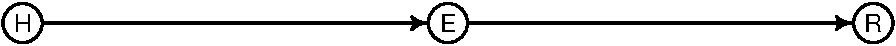
\includegraphics[width=0.5\linewidth,height=0.3\textheight]{ReplyToSteeleStefansson5_files/figure-latex/veracityDAG-1} \end{center}

\noindent As before, the hypothesis node \(H\) bears on the whereabouts
of the defendant and has two values, \textit{H=present} and
\textit{H=absent}. Note the difference between \(E\) and \(R\). The
evidence node \(E\) bears on the visual experience had by the witness.
The reporting node \(R\), instead, bears on what the witness reports to
have seen. The chain of transmission from `visual experience' to
`reporting' may fail for various reasons, such as lying or
misremembering.

In \textsc{Veracity}, the conditional probabilities,
\(\pr{E=e \vert H=h}\) should be the same as \(\ppr{+}{E=e \vert H=h}\)
for any values \(e\) and \(h\) of the variables \(H\) and \(E\) that are
shared before and after awareness growth. In comparing the old and new
Bayesian network, this equality falls out from their structure, as the
connection between \(H\) and \(E\) remains unchanged. Thus, constraint
(C)---along with Reverse Bayesianism---is perfectly fine in scenarios
such as \textsc{Veracity}.

This does not mean that the assessment of the probability of the
hypothesis \textit{H=present} should undergo no change. If you worry
that the witness could have lied, this should presumably make you less
confident about \textit{H=present}. To accommodate this intuition,
\textsc{Veracity} can be interpreted as a scenario in which an episode
of awareness refinement takes place together with a form of retraction.
At first, after the learning episode, you update your belief based on
the \textit{visual experience} of the witness. But after the growth in
awareness, you realize that your learning is in fact limited to what the
witness \textit{reported} to have seen. The previous learning episode is
retracted and replaced by a more careful statement of what you learned:
instead of conditioning on \textit{E=seen}, you should condition on what
the witness reported to have seen, \textit{R=seen-reported}. This
retraction will affect the probability of the hypothesis
\textit{H=present}.

Where does this leave us? Refinement cases that might at first appear
similar can be structurally different in important ways, and this
difference can be appreciated by looking at the Bayesian networks used
to model them. In modeling \textsc{Veracity}, the new node is added
downstream, while in modeling \textsc{Lighting}, it is added upstream.
This difference affects how probability assignments should be revised.
Since the conditional probabilities associated with the upstream nodes
are unaffected, Reverse Bayesianism is satisfied in
\textsc{Veracity}.\footnote{Note that
  \(\pr{\textit{H=present}\vert \textit{E=seen}}\neq \pr{\textit{H=present}\vert \textit{R=seen-reported}}\),
  but since you are conditioning on different propositions, this does
  not conflict with Reverse Bayesianism.} By contrast, since the
conditional probabilities associated with the downstream node will often
have to change, Reverse Bayesianism fails in \textsc{Lighting}.

This further corroborates our working hypothesis: structural features
about how we conceptualize a specific scenario are the guiding
principles about how we update the probability function through
awareness growth, not a formal principle like Reverse Bayesianism. We
further elaborate on this conjecture by drawing on some examples from
Anna Mathani.

\hypertarget{sure-no-gain-bets}{%
\subsection{Sure no-gain bets}\label{sure-no-gain-bets}}

Suppose the witness reports to have seeing the defendant around the
crime scene. You are not aware that the witness could be lying. Thus,
you are 100\% confident that the witness saw is what they report to have
seeing. In fact, you make no distinction between reporting to have
seeing and seeing itself. So you would be willing to buy for 1\$ the
following bet: if the witness saw the defendant, you get 1\$, and 0\$
otherwise. If the witness did see the defendant, you get you 1\$ back,
and otherwise you loose \textbackslash1\$. You are 100\% sure the
witness did see the defendant, so---by your lights---you stand to loose
no money whatsoever from this bet. But suppose that, as a matter of
fact, there is a difference between reporting and seeing. So,the witness
might report to have seeing something without actually having seeing it.
So, contrary to your conviction, that the witness saw the defendant is
not 100\% probable. This means that you would be willing to engage in a
bet in which you are guaranteed not to win any money and could
potentially lose money. If the witness did see the defendant you would
get your 1\$ back, but if not, you would lose it.

\hypertarget{mathanis-counterexamples}{%
\section{Mathani's counterexamples}\label{mathanis-counterexamples}}

\label{sec:mathani}

Mathani (2020) offers two counterexamples to Reverse Bayesianism. The
first goes like this:

\begin{quote}
\textsc{Tenant}: Suppose that you are staying at Bob's flat which he shares with his landlord. You know
that Bob is a tenant, and that there is only one landlord, and that this landlord also
lives in the flat. In the morning you hear singing coming from the shower room, and
you try to work out from the sounds who the singer could be. At this point you have
two relevant propositions that you consider possible ... $Landlord$ standing for the possibility that the landlord is the singer, and $Bob$ standing for the possibility that Bob is the singer  \dots  Because you know that Bob is a tenant in the flat, you also have a credence in the proposition $Tenant$ that the singer is a tenant. Your credence in $Tenant$ is the same as your credence in $Bob$, for given your state of awareness these two propositions are equivalent ... Now let's suppose the possibility suddenly occurs to you that there might be another tenant living in the same flat  ($Other$).
\end{quote}

\doublespace

\noindent Initially, you thought the singer could either be the landlord
or Bob, the tenant. Then you come to the realization that a third person
could be the singer, another tenant. Before awareness growth, that Bob
is in the shower and that a tenant is in the shower are equivalent
descriptions. After awareness growth, this equivalence breaks down.

Why is this scenario problematic? Suppose, after you hear singing in the
shower, you become sure someone is in there, but you cannot tell who. So
\(\pr{Landlord} = \pr{Bob} = 1/2\), and since \(Bob\) and \(Tenant\) are
equivalent, also \(\pr{Tenant}\) = 1/2. Now, \(Landlord\), \(Bob\) and
\(Tenant\) are all propositions that you were originally aware of, and
thus Reverse Bayesianisn requires that their assigned probabilities
should remain in the same proportion after your awareness grows. But
note that \(Other\) entails \(Tenant\) and \(Bob\) and \(Other\) are
disjoint, so it follows that \(\ppr{+}{Other}\) must have zero
probability.\footnote{If \(\ppr{+}{Other}>0\), the proportion of
  \(Tenant\) to \(Landlord\) or the proportion of \(Bob\) to
  \(Landlord\) should change.} This is an undesired outcome that rules
out the possibility that there could be a third person in the
shower.\footnote{Awareness Rigidity is no of help either because it
  would require that
  \(\ppr{+}{Landlord \vert Landlord \vee Tenant}=\ppr{+}{Bob \vert Landlord \vee Tenant}\)
  both equal \(1/2\), thus forcing
  \(\ppr{+}{Other \vert Landlord \vee Tenant}\) to zero.}

Consider now Mathani's second counterexample:

\begin{quote} 
\textsc{Coin}: You know that I am holding a fair ten pence UK coin which I am about to toss. You
have a credence of 0.5 that it will land $Heads$, and a credence of 0.5 that it will
land $Tails$. You think that the tails side always shows an engraving of a lion. So you
also  have a credence of 0.5 that ($Lion$) it will land with the lion engraving face-up: relative to your state of awareness $Tails$ and $Lion$ are equivalent.... Now let's suppose that you somehow become aware
that occasionally ten pence coins have .... an engraving of Stonehenge on the tails side. 
\end{quote}

\doublespace

\noindent  \(Tails\) and \(Lion\) are equivalent propositions prior to
awareness growth. Suppose you initially gave \(Tails\) and \(Lion\) the
same credence. Reverse Bayesianism requires that their relative
proportions should stay the same after awareness grow. The same applies
to \(Heads\) and \(Tails\). But since \(Lion\) and \(Stonehenge\) are
incompatible and the latter entails \(Tails\), you should have
\(\ppr{+}{Stonehenge} = 0\), again an undesirable conclusion.

Mathani notes that \textsc{Coin} has the same structure as
\textsc{Tenant}. This is true to some extent, but there is also an
interesting asymmetry between the two scenarios. In \textsc{Tenant}, it
is natural to assign \(1/3\) to \(Landlord\), \(Bob\) and \(Other\)
after awareness growth. That someone is singing in the shower is
evidence that someone must be in there, but without any more
discriminating evidence, each person should be assigned the same
probability. Consequently, a probability of 2/3 should be assigned to
\(Tenant\). On this picture, the proportion of \(Landlord\) to
\(Tenant\) changes from 1:1 (before awareness growth) to 1:2 (after
awareness growth). But, in \textsc{Coin}, the relative proportion of
\(Heads\) to \(Tails\) should remain constant throughout, unless
evidence emerges that the coin is not fair. One might have expected that
\(Landlord\) and \(Tenant\) would behave just like \(Heads\) and
\(Tails\), but actually they do not.

Bayesian networks can help to model the asymmetry between these two
scenarios. Consider \textsc{Coin} first. The structure of the scenario
is represented by the following graph:

\begin{center}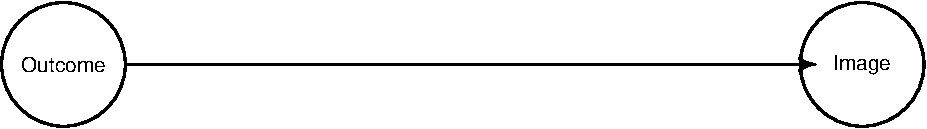
\includegraphics[width=0.5\linewidth,height=0.3\textheight]{ReplyToSteeleStefansson5_files/figure-latex/tailsDAG-1} \end{center}

\noindent The upstream node \(Outcome\) has two states, \(tails\) and
\(heads\). These two states remain the same throughout. What changes are
the states associated with the \(Imagine\) node downstream. Before
awareness growth, the node \(Image\) has two states: \(lions\) and
\textit{heads-image}.\footnote{The heads side must have some image, not
  specified in the scenario.} You assume that \(Image=lions\) is true if
and only if \(Outcome=tails\) is true. Then, you come to the realization
that the imagines for tails include a lion or a stonehenge engraving.
So, after awareness growth, the node \(Image\) contains three states:
\(lion\), \(stonehenge\) and \textit{heads-image}. Consider now the
other scenario, \textsc{Tenant}. We start with the following graph:

\begin{center}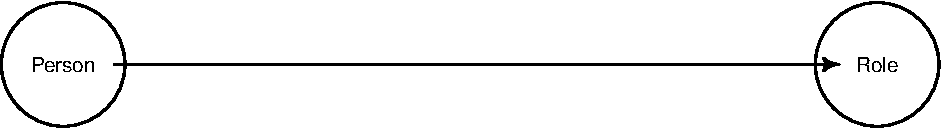
\includegraphics[width=0.5\linewidth,height=0.3\textheight]{ReplyToSteeleStefansson5_files/figure-latex/tenantsDAG-1} \end{center}

\noindent Initially, the upstream node \(Person\) has two possible
states, representing who is in the bathroom singing:
\textit{landlord-person} and \(bob\). To simplify things, the assumption
here is that the evidence of singing has already ruled out the
possibility that no one would be in the shower. The downstream node
\(Role\) has also two values, \(landlord\) and \(tenant\). After your
awareness grows, the upstream node \(Person\) should now have one more
possible state, \(other\).

The difference in modeling the two scenarios is this. In \textsc{Coin},
the states of the upstream node remain fixed, whereas in
\textsc{Tenant}, they change. After awareness growth, no new state is
added to \(Outcome\), but an additional state, \(other\), is added to
\(Person\). Plausible probability distributions for the Bayesian
networks associated with the two scenarios are displayed in Table
\ref{table:coin-tenant}. How the networks should be built and which
probabilities should shift is based on our background knowledge. This
knowledge tells us that the equiprobability of \(heads\) and \(tails\)
should not be affected by realizing that \(stonhenge\) is another
possible engraving for the tails side. It also tells us that the
probabilities of \(landlord\) and \(tenant\) should be affected by
realizing that a third person could be in the shower.

We conclude with some programmatic remarks. We think that the awareness
of agents grows while holding fixed certain material structural
assumptions, based on commonsense, semantic stipulations or causal
dependency.\footnote{Arrows in Bayesian networks are often taken to
  represent causal relationships, but other interpretations exist.
  Schaffer (2016) discusses an interpretation in which arrows represent
  grounding relations rather than causality. \label{footnote:causation}}
To model awareness growth, we need a formalism that can express these
material structural assumptions. This can done using Bayesian networks,
and we offered some illustrations of this strategy. These material
assumptions also guide us in formulating the adequate conservative
constraints, and these will inevitably vary on a case-by-case basis. The
literature on awareness growth from a Bayesian perspective is primarily
concerned with a formal, almost algorithmic solution to the problem.
Insofar as Reverse Bayesianism is an expression of this formalistic
aspiration, we agree with Steele and Stefánsson that we are better off
looking elsewhere.

\begin{table}
\begin{tabular}{clcc}
$\pr{Image \vert Outcome}$ & & \multicolumn{2}{c}{$Outcome$} \\
 &   & $heads$ & $tails$ \\
\multirow{2}{*}{$Image$} & $lion$ & 0 & 1\\
& \textit{heads-image} & 1 & 0 \\
\hline
\hline
$\ppr{+}{Image \vert Outcome}$ & & \multicolumn{2}{c}{$Outcome$} \\
&  & $heads$ & $tails$ \\
\multirow{3}{*}{$Image$} & $lion$ & 0 & 1/2\\ 
& $stonehenge$ & 0 & 1/2 \\
& \textit{heads-image} & 1 & 0 \\
\hline
\hline
$\pr{Outcome}=\ppr{+}{Outcome}$ & \multicolumn{2}{c}{$Outcome$} & \\
&  $heads$ & $tails$ & \\
& 1/2 & 1/2 & \\
\end{tabular}


\begin{tabular}{clccc}
&&&&\\
&&&&\\
$\pr{Role \vert Person}$ & & \multicolumn{3}{c}{$Person$} \\
 &   & \textit{landlord-person}  & \multicolumn{2}{c}{$bob$} \\
\multirow{2}{*}{$Role$} & $tenant$ & 0 & \multicolumn{2}{c}{1}\\
& $landlord$  & 1 & \multicolumn{2}{c}{0} \\
\hline
\hline
$\ppr{+}{Role \vert Person}$ & & \multicolumn{3}{c}{$Person$} \\
&  & \textit{landlord-person} & $bob$ & $other$ \\
\multirow{2}{*}{$Role$} & $tenant$ & 0 & 1/2 & 1/2\\ 
& $landlord$ & 1 & 0 & 0 \\
\hline
\hline
$\pr{Person}$ & \multicolumn{2}{c}{$Person$} & \\
&  \textit{landlord-person} & $bob$ & \\
& 1/2 & 1/2 & \\
\hline
\hline
$\ppr{+}{Person}$ & \multicolumn{2}{c}{$Person$} & \\
&  \textit{landlord-person} & $bob$ & $other$ \\
& 1/3 & 1/3 & 1/3 \\
\end{tabular}
\caption{Top table displays a plausible probability distribution for \textsc{Coin} and bottom table does the same for \textsc{Tenant}.}
\label{table:coin-tenant}
\end{table}

\hypertarget{towards-a-general-theory}{%
\section{Towards a general theory}\label{towards-a-general-theory}}

Awareness growth can occur in different ways. The key question is to
what extent probability assignments that were made prior to the episode
of awareness growth can be retained. There seems to no clear rule that
can decide that. We propose the following procedure. Construct a
Bayesian network prior to awareness growth and compare it with the new
Bayesian network after awareness growth. If the new arrows and nodes are
all downstream, the old probabilities table should not be changed. The
paradigmatic cases of this are scenarios \textsc{Veracity} and
\textsc{Coin}. If, instead, the new arrows and and nodes are upstream,
the old probabilities tables should be changed. The paradigmatic
examples are \textsc{Lighting} and \textsc{Tenant}.

\hypertarget{counterexamples}{%
\section{Counterexamples}\label{counterexamples}}

In this section, we rehearse two of the counterexamples to Reverse
Bayesianism by Steele and Stefánsson. One example targets awareness
expansion and the other awareness refinement (more on this distinction
soon). We show why they make a limited case against Reverse Bayesianism
and then provide a better counterexample with the aid of Bayesian
networks.

\hypertarget{friends-and-movies}{%
\subsection{Friends and Movies}\label{friends-and-movies}}

\label{sec:counterexamples}

The difference between expansion and refinement is intuitively
plausible, but can be tricky to pin down formally. A rough
characterization will suffice here. Suppose, as is customary,
propositions are interpreted as sets of possible worlds, where the set
of all possible worlds is the possibility space. An algebra of
propositions thus interpreted induces a partition of the possibility
space. Refinement occurs when the new proposition added to the algebra
induces a more fine-grained partition of the possibility space.
Expansion occurs when the new proposition is inconsistent with the
existing ones, thus making the old partition no longer exhaustive.

This is not the end of the story, however. Steele and Stefánsson offer
another counterexample that also works against Awareness Rigidity, this
time targeting a case of refinement:

\begin{quote}
\textsc{Movies}: Suppose you are deciding whether to see a movie at your
local cinema. You know that the movie's predominant language and genre
will affect your viewing experience. The possible languages you consider
are French and German and the genres you consider are thriller and
comedy. But then you realise that, due to your poor French and German
skills, your enjoyment of the movie will also depend on the level of
difficulty of the language. Since it occurs to you that the owner of the
cinema is quite simple-minded, you are, after this realisation, much
more confident that the movie will have low-level language than
high-level language. Moreover, since you associate low-level language
with thrillers, this makes you more confident than you were before that
the movie on offer is a thriller as opposed to a comedy. (Steele \&
Stefánsson, 2021, sec. 5, Example 3)
\end{quote}

\doublespace

\noindent This is a case of refinement. For you initially categorized
movies by just language and genre, and then you refined your
categorization by adding another variable, level of difficulty. Without
considering language difficulty, you assigned the same probability to
the hypotheses \textit{Thriller} and \textit{Comedy}. But learning that
the owner was simple-minded made you think that the level of linguistic
difficulty must be low and the movie most likely a thriller rather than
a comedy (perhaps because thrillers are simpler---linguistically---than
comedies). So, against Reverse Bayesianism, \textsc{Movies} violates the
condition
\(\frac{\pr{\textit{Thriller}}}{\pr{\textit{Comedy}}}=\frac{\ppr{+}{\textit{Thriller}}}{\ppr{+}{\textit{Comedy}}}\).

The counterexample also violates Awareness Rigidity. For consider a
proposition that picks out the entire possibility space, for example,
\(\textit{Thriller}\vee \textit{Comedy}\).\footnote{Since
  \textsc{Movies} is a case of refinement,
  \(\textit{Thriller}\vee \textit{Comedy}\) picks out the entire
  possibility space both before and after awareness growth.} Awareness
Rigidity would require that
\(\pr{\textit{Thriller}}=\ppr{+}{\textit{Thriller} \vert \textit{Thriller}\vee \textit{Comedy}}\).
But \textsc{Movies} does not satisfy this equality since the probability
of \textit{Thriller} has gone up.

How good of a counterexample is this? Steele and Stefánsson consider an
objection:

\begin{quote}It might be argued that our examples are not illustrative of \dots a simple growth in awareness; rather, our examples illustrate and should be expressed 
  formally as complex learning experiences, where first there is a growth in awareness, and then 
  there is a further learning event ... In this way, one could argue that the awareness-growth 
  aspect of the learning event always satisfies Reverse Bayesianism.
\end{quote}

\doublespace

\noindent  Admittedly, \textsc{Movies} can be split into two episodes.
In the first, you entertain a new variable besides language and genre,
namely the language difficulty of the movie. In the second episode, you
learn something you did not consider before, namely that the owner is
simple-minded. Could Reserve Bayesianism still work for the first
episode, but not the second? Steele and Stefánsson do not address this
question explicitly, but insist that no matter the answer both episodes
are instances of awareness growth. We agree with them on this point.
Awareness growth is both \textit{entertaining} a new proposition not in
the initial awareness state of the agent and \textit{learning} a new
proposition. Nonetheless, many could still wonder. Is the second episode
(learning something new) necessary for the counterexample to work
together with the first episode (mere refinement without learning)?

Suppose the counterexample did work only in tandem with an episode of
learning something new. If that were so, defenders of Reverse
Bayesianism or Awareness Rigidity could still claim that their theory
applies to a large class of cases. It applies to cases of awareness
refinement without learning and also to cases of awareness expansion.
For recall that the first putative counterexample featuring awareness
expansion---\textsc{Friends}---did not challenge Reverse Bayesianism
insofar as the latter is formulated in terms of its close cousin,
Awareness Rigidity. So the force of Steele and Stefánsson's
counterexamples would be rather limited.

\singlespace

\hypertarget{references}{%
\section*{References}\label{references}}
\addcontentsline{toc}{section}{References}

\hypertarget{refs}{}
\begin{CSLReferences}{1}{0}
\leavevmode\vadjust pre{\hypertarget{ref-bradley2017}{}}%
Bradley, R. (2017). \emph{Decision theory with a human face}. Cambridge
University Press.

\leavevmode\vadjust pre{\hypertarget{ref-chihara1987}{}}%
Chihara, C. S. (1987). Some problems for bayesian confirmation theory.
\emph{British Journal for the Philosophy of Science}, \emph{38}(4),
551--560.

\leavevmode\vadjust pre{\hypertarget{ref-eerman1992}{}}%
Earman, J. (1992). \emph{Bayes or bust? A critical examination of
bayesian confirmation theory}. MIT press.

\leavevmode\vadjust pre{\hypertarget{ref-fenton2013GeneralStructureLegal}{}}%
Fenton, N., Neil, M., \& Lagnado, D. A. (2013). A {General Structure}
for {Legal Arguments About Evidence Using Bayesian Networks}.
\emph{Cognitive Science}, \emph{37}(1), 61--102.
\url{https://doi.org/10.1111/cogs.12004}

\leavevmode\vadjust pre{\hypertarget{ref-glymour1980}{}}%
Glymour, C. (1980). \emph{Theory and evidence}. Princeton University
Press.

\leavevmode\vadjust pre{\hypertarget{ref-howson1976}{}}%
Howson, C. (1976). The development of logical probability. In
\emph{Essays in memory of imre lakatos. Boston studies in the philosophy
of science} (pp. 277--298). Springer.

\leavevmode\vadjust pre{\hypertarget{ref-karniViero2015}{}}%
Karni, E., \& Vierø, M.-L. (2015). Probabilistic sophistication and
reverse bayesianism. \emph{Journal of Risk and Uncertainty Volume},
\emph{50}, 189--208.

\leavevmode\vadjust pre{\hypertarget{ref-lakatos1968}{}}%
Lakatos, I. (1968). Changes in the problem of inductive logic.
\emph{Studies in Logic and the Foundations of Mathematics}, \emph{51},
315--417.

\leavevmode\vadjust pre{\hypertarget{ref-mathani2020}{}}%
Mathani, A. (2020). Awareness growth and dispositional attitudes.
\emph{Synthese}, \emph{198}(9), 8981--8997.

\leavevmode\vadjust pre{\hypertarget{ref-Pettigrew2022}{}}%
Pettigrew, R. (forthcoming). How should your beliefs change when your
awareness grows? \emph{Episteme}, 1--25.
\url{https://doi.org/10.1017/epi.2022.33}

\leavevmode\vadjust pre{\hypertarget{ref-roussos2021}{}}%
Roussos, J. (2021). Awareness growth and belief revision.
\emph{Manuscript}.

\leavevmode\vadjust pre{\hypertarget{ref-schaffer2016}{}}%
Schaffer, J. (2016). Grounding in the image of causation.
\emph{Philosophical Studies}, \emph{173}, 49--100.

\leavevmode\vadjust pre{\hypertarget{ref-steeleStefansson2021}{}}%
Steele, K., \& Stefánsson, O. (2021). Belief revision for growing
awareness. \emph{Mind}, \emph{130}(520), 1207--1232.

\leavevmode\vadjust pre{\hypertarget{ref-wenmackersRomeijn2016}{}}%
Wenmackers, S., \& Romeijn, J.-W. (2016). New theory about old evidence:
A framework for open-minded bayesianism. \emph{Synthese Volume},
\emph{193}, 1225--1250.

\leavevmode\vadjust pre{\hypertarget{ref-williamson2003}{}}%
Williamson, J. (2003). Bayesianism and language change. \emph{Journal of
Logic, Language, and Information}, \emph{12}(1), 53--97.

\leavevmode\vadjust pre{\hypertarget{ref-zabell1992}{}}%
Zabell, S. (1992). Predicting the unpredictable. \emph{Synthese},
\emph{90}(1), 205--232.

\end{CSLReferences}

\end{document}
